\chapter{Solução Proposta}
\label{cap:solucao}

Considerando os requisitos de coreografias de serviços web, de uso da computação em nuvem e de sistemas em grande escala, projetamos e implementamos um arcabouço de middleware para a implantação de coreografias de serviços web denominado CHOReOS \ee. Os serviços oferecidos pelo nosso arcabouço integram-se ao Ambiente Integrado de Desenvolvimento e Execução CHOReOS, que visa fornecer todo o processo de desenvolvimento, implantação e governança de coreografias de serviços web. Para a implementação do arcabouço Enactment Engine contribuíram Daniel Cuckier, Carlos Eduardo do Santos, Felipe Pontes, Alfonso Diaz, Nelson Lago, Paulo Moura, Thiago Furtado e demais colegas dos projetos Baile e CHOReOS. O código-fonte do \ee\ é software livre 
sob a Licença Pública da Mozilla 2\footnote{\url{http://www.mozilla.org/MPL/2.0/}} 
e está disponível em \url{http://ccsl.ime.usp.br/enactmentengine}. 

Neste capítulo, descrevemos a arquitetura do arcabouço proposto, incluindo os pontos de extensão previstos. Destacamos os aspectos cobertos e não cobertos dos requisitos de sistemas de grande escala. Apresentamos também o estado atual da implementação do arcabouço, assim como os resultados experimentais sobre sua escalabilidade obtidos até o momento.

\section{Arquitetura}

\todo{atenção, estaremos utilizando a nomenclatura do DEPL, como definida no cap 2}

A arquitetura do \ee é exibida na Figura~\ref{fig:arquitetura}.
\todo{quais fizemos e quais são prontos}

\begin{figure}[ht]
\centering
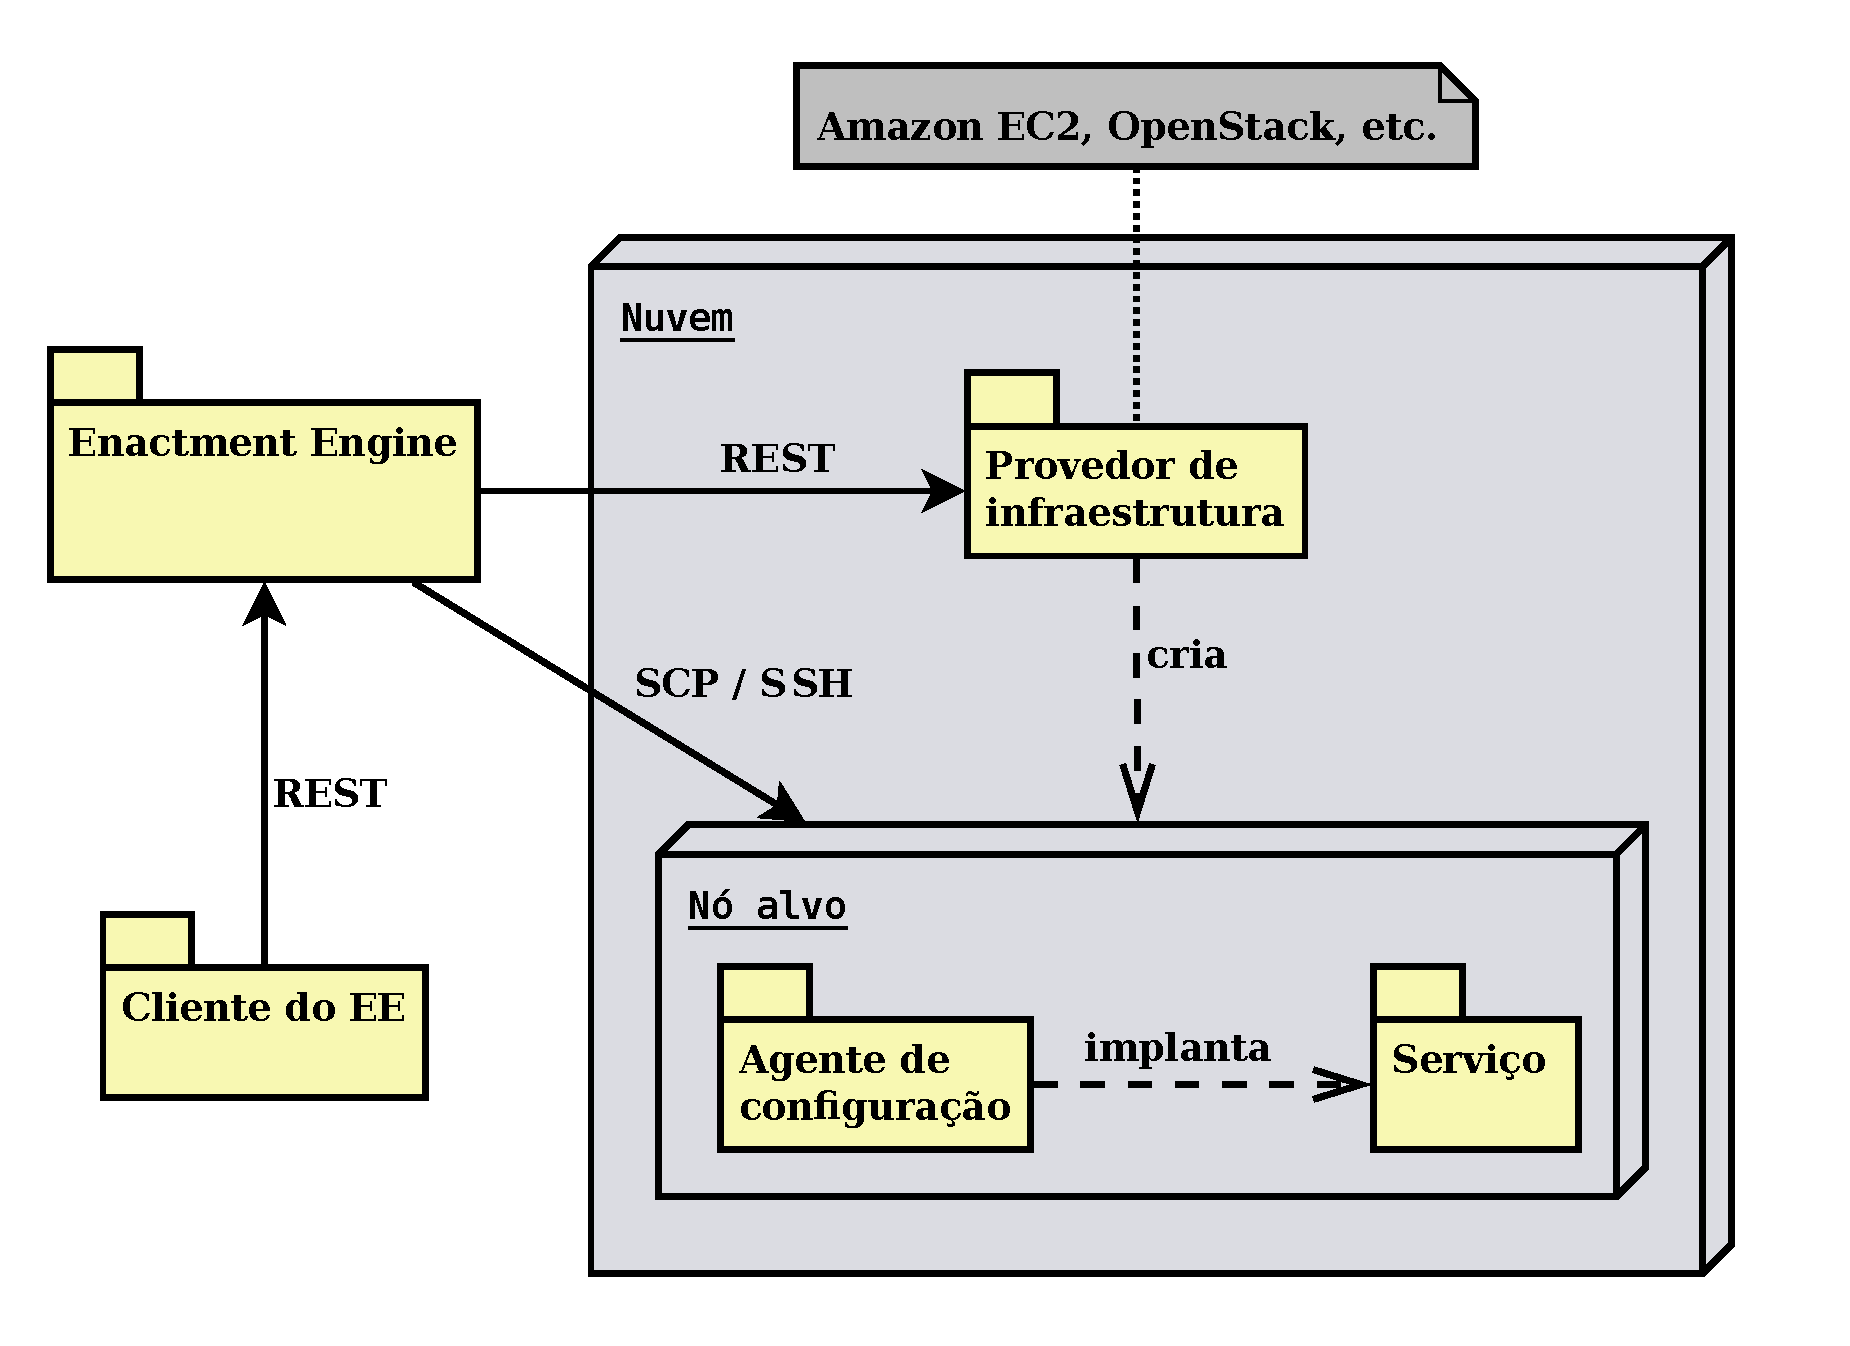
\includegraphics[width=0.7\linewidth]{arquitetura.pdf}
\caption{Arquitetura do \choreos \ee.}
\label{fig:arquitetura}
\end{figure}

\begin{itemize}

\item O \emph{Cloud Gateway} é um serviço capaz de criar e destruir máquinas virtuais (também chamadas de \emph{nós}), normalmente em um ambiente de computação em nuvem. Atualmente o \ee suporta o Amazon EC2 e o OpenStack.

\item O \emph{agente de configuração} é executado nos nós alvos
e dispara os scripts que implementam as fases de preparação
e inicialização da implantação dos serviços.
O \ee utiliza o Chef Solo\footnote{\url{http://docs.opscode.com/chef_solo.html}}
como seu agente de configuração.

\item O \emph{\ee} em si...

%
%\item The \emph{\dm} deploys services in a cloud environment. 
%	It receives a declarative service specification and creates or selects the
%    node onto which the service will be deployed, possibly considering service
%    non-functional requirements. The \dm\ converts the received specification
%    into scripts that prepares and execute the service
%    processes. It also runs the Configuration Agent on the target nodes,
%    where services are actually deployed. 
%    Each \dm\ is associated with a cloud infrastructure account.
%
%\item The \emph{\cd}, based on a choreography specification, 
%    coordinates invocations to multiple \dm{s}
%    belonging to participant organizations. When services are
%    already running, the \cd\ performs \emph{service binding}, 
%    so participant services are informed about the location of each other.
%

\item O \emph{cliente do \ee} ...

\end{itemize} 

A Figura~\ref{fig:processo} exibe o processo de implantação de composições
de serviços implementado pelo \ee:

\begin{figure}[ht]
\centering
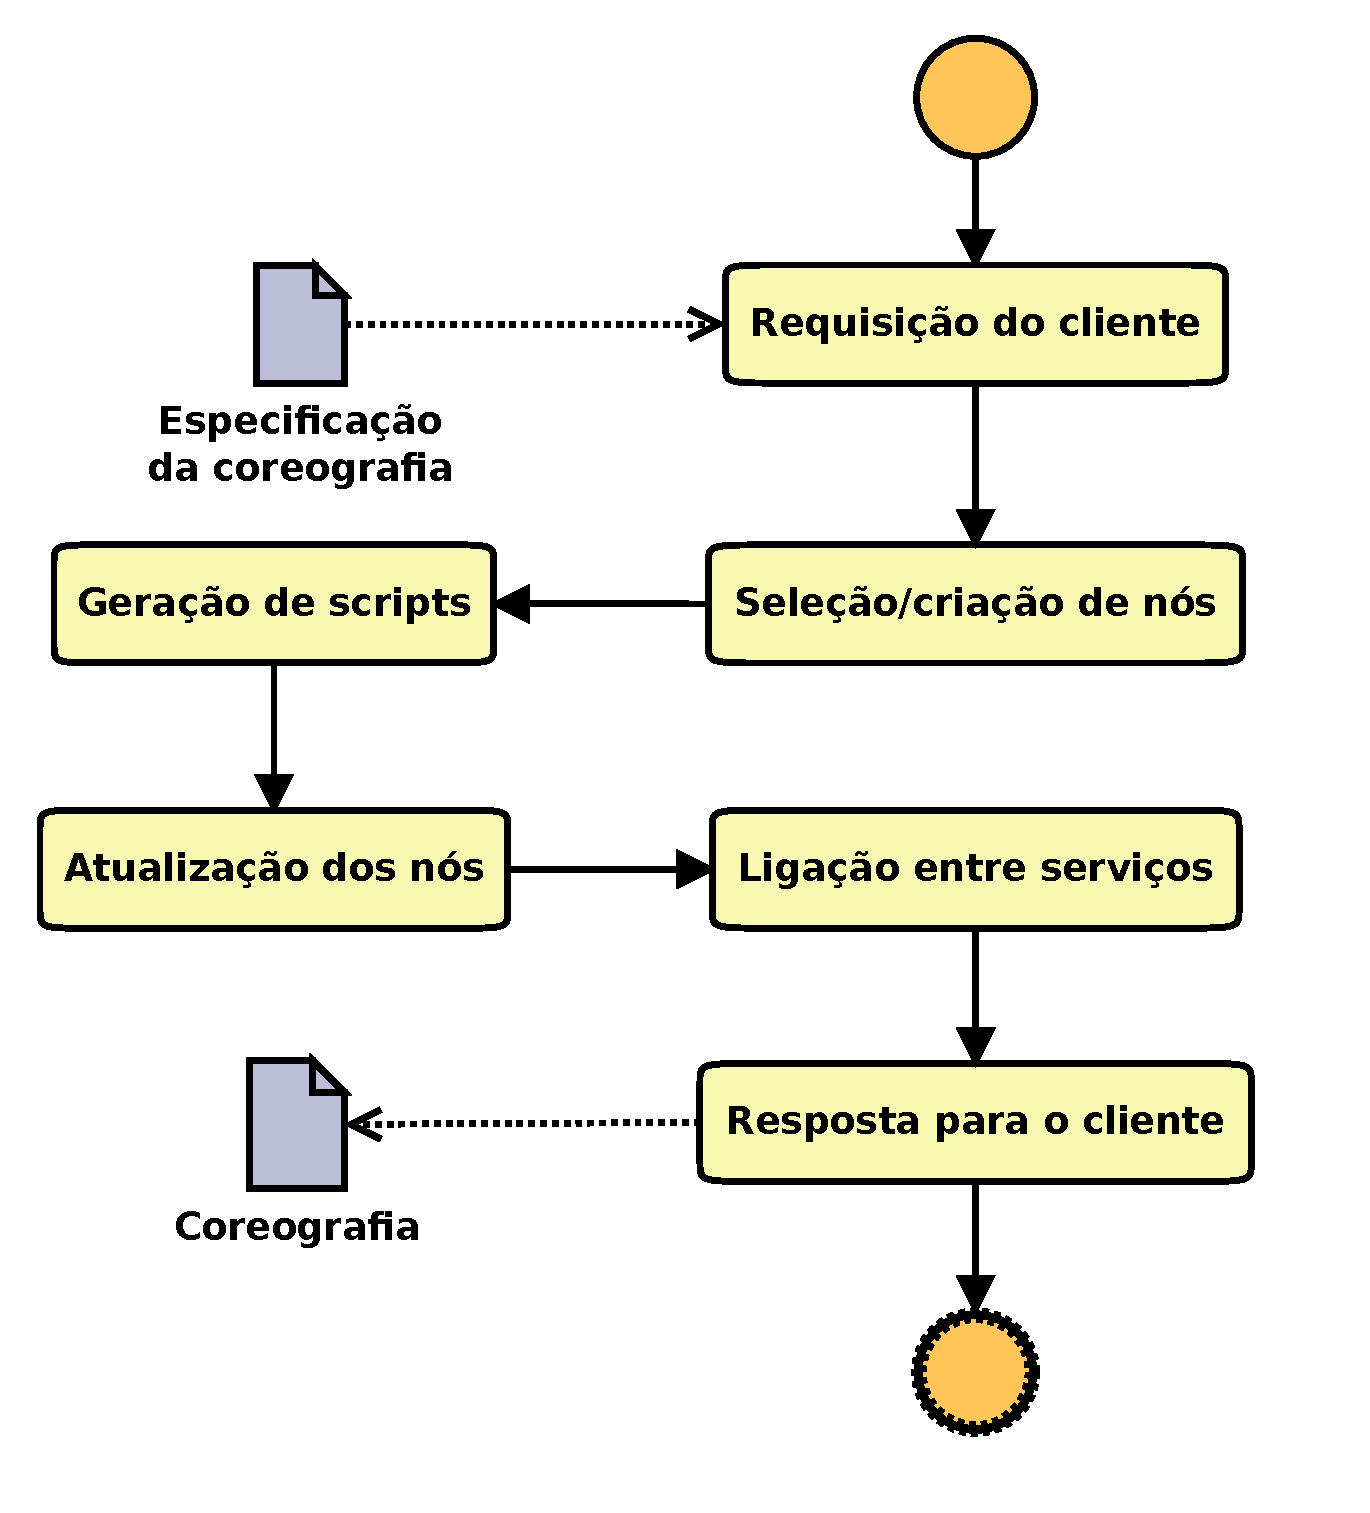
\includegraphics[width=0.5\textwidth]{processo.pdf}
\caption{Processo de implantação implementado pelo \ee.}
\label{fig:processo}
\end{figure}

\begin{enumerate}
\item \emph{Requisição do cliente:}
\item \emph{Seleção/criação de nós}:
\item \emph{Geração de scripts}:
\item \emph{Atualização dos nós}:
\item \emph{Ligação entre serviços}:
\item \emph{Resposta para o cliente}:

%\item \emph{Client request:} receives the specification of the service composition to be deployed.
%\item \emph{Node selection:} selects one or more cloud nodes where each service will be deployed, creating new nodes if necessary and accommodating service non-functional requirements.
%\item \emph{Scripts generation:} dynamically creates scripts for environment configuration and service launching. 
%\item \emph{Nodes update:} executes the scripts on the selected nodes, so that services are installed and launched.
%\item \emph{Service binding:} injects addresses of service dependencies (other participant services in the composition).
%\item \emph{Response to client:} sends the response to the client, informing which services were deployed in which nodes, and the service URIs enabling runtime monitoring.
\end{enumerate}

%Additionally, there are optional steps such as setting up a monitoring infrastructure, both at cloud resource and service level. To monitor cloud resources (e.g., VM memory, CPU, and network usage), the \EE installs a monitoring agent (Ganglia\footnote{\url{http://ganglia.sourceforge.net}}) in each node. To perform service-level monitoring, services may be bound automatically to a distributed Enterprise Service Bus node (EasyESB\footnote{\url{https://research.petalslink.org/display/easyesb}}).


\section{Interface}

\section{Pontos de extensão}

\section{Aspectos gerais de implementação}

\section{Aspectos da implementação que auxiliam na superação dos desafios de implantação de sistema de grande escala}
